\chapter{The Raman effect}
\label{ch:Raman}

This chapter explains how to understand the Raman-effect. Link to Desmos notebooks. 

\section{Microscopic picture}
When exposed to an oscillating electromagnetic field, the electrons in the medium will respond almost instantly due to their low mass. The nuclei around which these electrons orbit will react much more slowly due to their comparatively large mass. The result is that the nonlinear phase shift affecting a particular instant of a pulse for a certain fiber segment depends on two things: The optical power of the pulse at that instant and the optical power that affected that location in the past. The nonlinear impact that time-delayed mechanical vibrations of the nuclei in the material lattice have on the electromagnetic field that induced them is called the "Raman effect" \CITE.  



\section{The Raman response function}
Mathematically, the impact of the Raman effect on an optical pulse can be described by
\begin{align}
\label{eq:raman}
 \partial_z \A = i\gamma\left( 
\A \int_{0}^{\infty} R(T_{delay})|\A(z,T-T_{delay})|^2 dT_{delay} \right),
\end{align}
which is equivalent to Eq.~\ref{eq:GNLSE} when attenuation, dispersion and self-steepening are ignored. The function, $R(T_{delay})$ is the total response function, which indicates how much the power at different times in the past contribute to the nonlinear phase shift affecting the pulse at a given instant. It can be written as the sum of an instantaneous contribution from the electronic response via a delta function and a delayed Raman response due to lattice vibrations as
\begin{align}
    \label{eq:response}
    R(T_{delay})&= (1-f_R)\delta(T_{delay})+f_Rh_R(T_{delay}),
\end{align}
where $0\leq f_R\leq 1$ is a scalar that determines the relative magnitude of the two contributions. The exact functional form of the Raman response function, $h_R(T_{delay})$, depends on the material, but generally resembles a sine function multiplied by a dampening term and must satisfy $\int_{-\infty}^{\infty}h_R(T_{delay}) dT_{delay}=1$, as it essentially "weighs" how much the powers at different times in the past contribute to the current nonlinear phase shift. Additionally, it must be demanded that $h_R(T_{delay})=0$ for $T_{delay}\leq0$ to prevent the expression from violating causality by letting \emph{future} powers affect the current nonlinear phase shift. 
Intuitively, the function $h_R(T_{delay})$ is like the function that describe the amplitude of a sound wave from a tuning fork, piano key or guitar string after it is suddenly struck; an oscillation that gradually "rings down". Continuing the analogy, if one views $|\A(z,T-T_{delay})|^2$ as a large collection of instantaneous strikes with different strengths at different times, it makes sense that the current oscillation depends on all the ones that were present in the past.  
Substituting Eq.~\ref{eq:response} into Eq.~\ref{eq:raman} and evaluating the integral over the delta function yields
\begin{align}
    \label{eq:raman_split}
    \partial_z \A = i\gamma\A\left( 
(1-f_R)|\A(z,T)|^2+f_R \int_{0}^{\infty} h_R(T_{delay})|\A(z,T-T_{delay})|^2 dT_{delay} \right).
\end{align}
Note that if the change in the power of the pulse is very slow compared to the duration of the response function, one can approximate $h_R(T_{delay})\approx \delta(T_{delay})$ (or, equivalently, $|\A(z,T-T_{delay})|^2\approx|\A(z,T)|^2$), in which case Eq.~\ref{eq:SPM} is recovered. In other words, the Raman effect is only noticeable for pulses whose durations are close to the duration of the natural oscillations of the molecular lattice! Assuming that the pulse duration is noticeably longer than the duration of $h_R(T_{delay})$, so that its power for different time delays can be found by linearly extrapolating the present power and its gradient into the past, the integral in Eq.~\ref{eq:raman_split} can be written as 
\begin{align}
\label{eq:raman_approx}
    f_R \int_{0}^{\infty} h_R(T_{delay})|\A(z,T-T_{delay})|^2 dT_{delay} &\approx\\ \nonumber \quad\quad\quad f_R \int_{0}^{\infty} h_R(T_{delay})\left[ 
  |\A(z,T)|^2-T_{delay}\partial_T|\A(z,T)|^2 \right] dT_{delay} &=\\ \nonumber \quad\quad\quad  |\A(z,T)|^2f_R- \partial_T|\A(z,T)|^2 f_R\int_{0}^{\infty} T_{delay} h_R(T_{delay}) 
   dT_{delay}&=\\ \nonumber \quad\quad\quad  |\A(z,T)|^2f_R- \partial_T|\A(z,T)|^2 T_R &,
\end{align}
where $T_R$ is the average duration of the Raman response function scaled by $f_R$. Substituting the result of Eq.~\ref{eq:raman_approx} into Eq.~\ref{eq:raman_split} yields
\begin{align}
    \label{eq:raman_approx_applied}
\partial_z \A = i\gamma\A\left( 
|\A(z,T)|^2-T_R \partial_T|\A(z,T)|^2\right),
\end{align}
which contains the "usual" SPM term proportional to the current power and an additional term that depends in the time derivative of the power. For silica, $T_R\approx 3$~fs, so Eq.~\ref{eq:raman_approx_applied} will be valid for pulses longer than approximately 600~fs. The approximation applied in Eq.~\ref{eq:raman_approx} could be extended to include the second derivative of $|\A(z,T)|^2$ for increased accuracy. Recall from Eq.~\ref{eq:SPM_example} and Fig.~\ref{fig:chirp_profiles} that the "constant" SPM term causes a large decrease in the instantaneous frequency where the \emph{derivative} of the power is very positive. By the same logic, the Raman term in Eq.~\ref{eq:raman_approx_applied} will cause a large decrease in the the instantaneous frequency where the "derivative of the derivative" is very negative. In other words, the Raman effect will tend to cause a red-shift at the peak of the pulse without an equivalently large blue-shift elsewhere, thus making the entire pulse "more red"! Physically, the red-shift arises because an incident photon can lose some of its energy by exciting mechanical vibrations in the crystal lattice of the medium. 

\subsection{Expressions for $h_R(T_{delay})$}
An approximate expression for the Raman effect in silica, which assumes that the molecular vibrations are dominated by a single frequency is 
\begin{align}
\label{eq:raman_basic}
    h_R^{basic}(T_{delay})&= \left(\frac{1}{\tau_1^{2}}+\frac{1}{\tau_2^{2}} \right)\tau_1\exp\left(-\frac{T_{delay}}{\tau_2}\right)\sin\left(\frac{T_{delay}}{\tau_1}\right),
\end{align}
with $f_R=0.18$, $\tau_1=12.2$~fs and $\tau_2=32$~fs. All presented expressions for $h_R(T_{delay})$ are assumed to be zero for $T_{delay}\leq0$ to respect causality. Mathematically, this can be ensured through multiplication by the Heaviside step-function.

A more accurate approximation than Eq.~\ref{eq:raman_basic} to the vibrational behavior of silica is  
\begin{align}
\label{eq:raman_new}
    h_R^{better}(T_{delay})&= (1-f_b) h_R^{basic}(T_{delay})+f_b\frac{2\tau_b-T_{delay}}{\tau_b^2}\exp\left(-\frac{T_{delay}}{\tau_b}\right),
\end{align}
where $f_R=0.245$, $f_b=0.21$ and $\tau_b=96$~fs. The exact expression for the Raman response of silica is

\begin{align}
\label{eq:Raman_exact}
    h_R^{exact}(T_{delay})&=c^{-1}_{norm}\sum_{n=0}^{12}A_n\exp\left(- g_nT_{delay}-0.25G_n^2T^2_{delay}  \right)\sin\left(2\pi \nu_nT_{delay} \right),
\end{align}
where $f_R=0.18$ and the parameters $A_n$, $g_n$, $G_n$, and $\nu_n$ are listed in Tab.~\ref{tab:raman_coeffs} and $c_{norm}=3.75225$~ps so that $\int_0^\infty h_R^{exact}(T_{delay}) dT_{delay}=1$. A visualization of these three models of the Raman response of silica and their impacts on the same optical pulse is presented in Fig.~\ref{fig:raman_combined}. The imaginary parts of the Fourier Transforms of the different expressions for $h_R(T_{delay})$ are plotted in Fig.~\ref{fig:raman_combined}~b). Physically, these spectra imply that for a given optical frequency, the Raman effect will allow it to "steal" power from frequencies 13~THz above it and force it to "donate" power to frequencies 13~THz below it. For reasons similar to those addressed in Sec.~\ref{sec:KK_relations}, the real parts of the spectra (not shown) relate to the change in refractive index due to the Raman effect and allows one to determine the time delay it induces. From the maximum values of the curves shown in Fig.~\ref{fig:raman_combined}~b), the maximum Raman gain and thus the characteristic length over which the Raman effect becomes significant can be expressed as
\begin{align}
    g_{Raman} &= \frac{4}{3} \gamma f_R P_0 n(\omega_0)\cdot max(  Im\{ \FT \{ h_R(T_{delay}) \}(\omega) \} )\\ 
    L_{Raman} &= \frac{1}{g_{Raman}},
\end{align}
where $P_0$ is the maximum power of the pulse and $n(\omega_0)$ is the refractive index of the medium ($\approx 1.47$ for silica). 


See \href{https://www.youtube.com/playlist?list=PLdFybGSAoPnn6tnSmptR71zKAgcKsjIfi}{these video tutorials} for more information on the Raman effect.   

\begin{table}
\begin{center}
    \begin{tabular}{c|c|c|c|c}
    \label{tab:raman_coeffs}
        n  &$A_n$ & $g_n$ [fs] & $G_n$ [fs] & $\nu_n$ [THz]  \\ \hline
        0  &  1    &0.521       &1.562          &1.69   \\
        1  &  11.4 &1.163       &3.310          &3.00   \\
        2  &  36.67&1.749       &5.246          &6.93   \\
        3  &  67.67&1.624       &4.872          &10.87\\
        4  &  74   &1.352       &4.057          &13.88       \\
        5  &  4.5  &0.245       &0.734          & 14.90   \\
        6  &  6.8  &0.415       &1.244          & 18.33   \\
        7  &  4.6  &1.549       &4.647          & 20.74   \\
        8  &  4.2  &0.594       &1.784          & 23.79  \\
        9  &  4.5  &0.642       &1.928          & 25.05   \\
        10 &  2.7  &1.499       &4.497          & 27.88   \\
        11 &  3.1  &0.909       &2.728          & 32.38   \\
        12 &  3    &1.599       &4.797          &   36.42 
    \end{tabular}
    \caption{Table of parameters of the exact expression for the Raman response of silica in Eq.~\ref{eq:Raman_exact} modified from \cite{raman_exact}.  }
    \end{center}
\end{table}

\begin{figure}
    \centering
    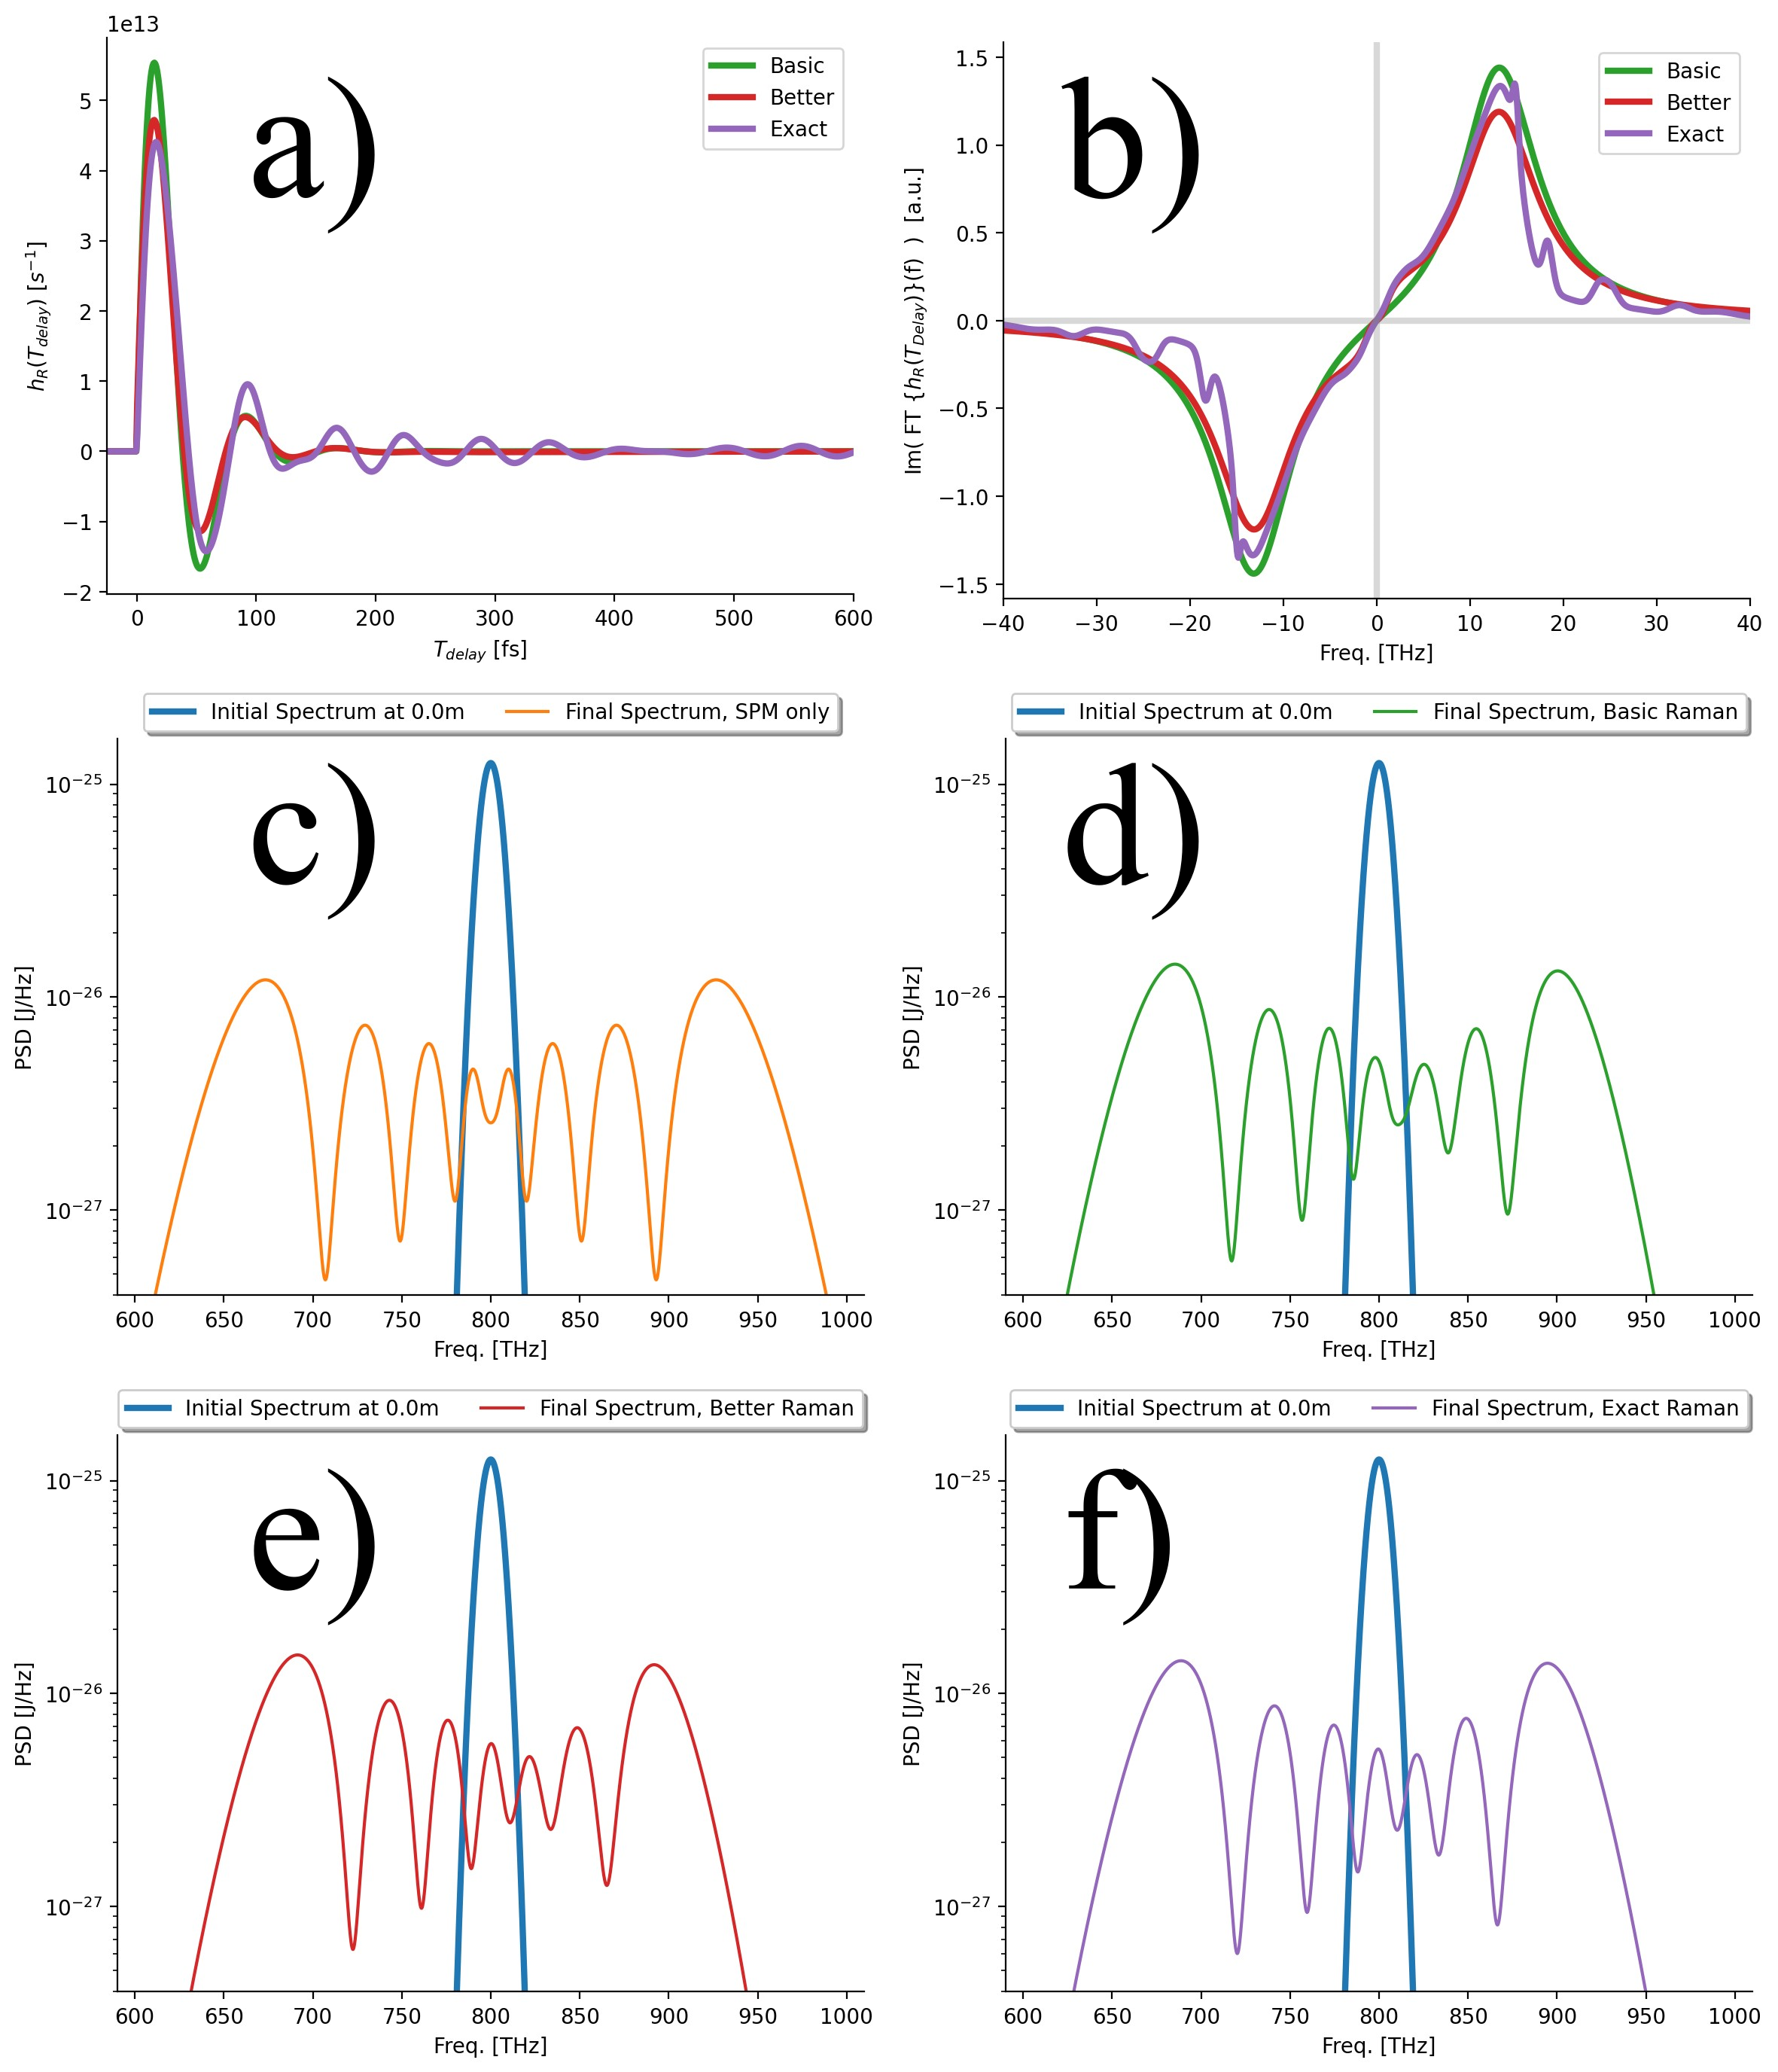
\includegraphics[width=1\linewidth]{figures/Raman_combined.png}
    \caption{a) Graphs of Eq.~\ref{eq:raman_basic} (green), Eq.~\ref{eq:raman_new} (red) and Eq.~\ref{eq:Raman_exact} (purple) in the time domain. b) Imaginary part of the Fourier Transform of the functions plotted in a). c) Initial and final spectrum of a pulse subjected to SPM only. d) Initial and final spectrum for the same pulse as in c) subjected to the Raman effect described by Eq.~\ref{eq:raman_basic}. Note the asymmetric broadening skewed to lower frequencies as predicted by the analysis of Eq.~\ref{eq:raman_approx_applied}. e) Same as d) but for Eq.~\ref{eq:raman_new} f) Same as d) but for Eq.~\ref{eq:Raman_exact}. Figures generated using \href{https://colab.research.google.com/drive/1TqixCGQ51DVwpB3VA6J1XQCpDcf4xwb4?usp=sharing}{this interactive notebook}, which the reader is encouraged to experiment with.}
    \label{fig:raman_combined}
\end{figure}




